\chapter{Using the EvA2 API\label{sec:Using-the-API}}

This chapter describes how to incorporate \noun{EvA2} into existing
projects through the Java API.


\section{Accessing Standard Optimizers\label{sub:Accessing-Standard-Optimizers}}

A standard optimizer is typically a well-known optimization algorithm
with operators and parameters predefined in a way so that a user may
start it out-of-the-box and expect good optimization results in general.
Of course, every expert may have an own notion on what parameters
are preferable in general. Therefore we give two customization examples
using the API. In any case, a necessary step is to extend a \noun{EvA2}
base class constituting the target function. You may, again, use the
\texttt{eva2.problems.simple} package described in Sec.~\ref{sec:Quickly-Adding-Your-Problem}.
However, this makes it necessary to use the wrapper class \texttt{SimpleProblemWrapper},
which is great for direct GUI usage but may make programming a bit
more complicated. We therefore, at this point, recommend to go one
step higher in hierarchy and extend \texttt{AbstractProblemDouble}
or \texttt{AbstractProblemBinary}.


\subsection{The Abstract Problem Classes\label{sub:The-Abstract-Problem-classes}}

The problem class subtree encapsulates properties of target functions
that can be directly optimized by the \noun{EvA2} framework and starts
at the \texttt{AbstractOptimizationProblem} class. The basic properties
of the problem class are functional: 
\begin{enumerate}
\item The problem is itself initialized, 
\item the problem knows how to initialize a set of potential solutions,
and 
\item the problem evaluates a set of potential solutions. 
\end{enumerate}
To implement your own target function in \noun{EvA2}, we recommend
inheriting from \texttt{AbstractProblemDouble} or \texttt{AbstractProblemBinary},
depending on your preferred data representation. Integer and program-data-based
problems are currently not covered by this document. Notice that if
you want your problem implementation to be displayed and manageable
by the GUI in the same way the predefined problems are handled, you
have to assign it the same package tree as its parent class (e.g.
\texttt{eva2.problems} for new problem implementations).


\paragraph*{The class \texttt{AbstractProblemDouble}}

The \texttt{AbstractProblemDouble} class in the package \texttt{eva2.prob\-lems}
encapsulates methods useful to implement double valued target functions.
Let's assume you want to implement a function $f_{\mathrm{target}}(x)=y$
with $f_{\mathrm{target}}:\;\mathbb{R}^{n}\rightarrow\mathbb{R}^{m}$.
Important for double-valued problems is the range of the solution
space, defining in any dimension the minimum and maximum value allowed.
By setting the \texttt{default\-Range} member variable (method \texttt{set\-Default\-Range})
in your constructor, you can easily define a symmetric range $[-dR,\; dR]^{n}$.
If you need a different range definition, you may overload the methods
\texttt{getRangeLowerBound(int dim)} and \texttt{getRangeUpperBound(int
dim)} which are to return the upper or lower range limit for a given
dimension.%
\begin{comment}
template? noise?
\end{comment}
{} 

The \texttt{AbstractProblemDouble} class also contains a noise parameter
and an individual template. The \emph{noise} can be used to add gaussian
fluctuation to any target function. If \emph{noise} > 0, it defines
the standard deviation of the random disturbance of $f_{\mathrm{target}}(x)$.
The individual template defines the data representation for potential
solutions. It also contains evolutionary operators which work directly
on the representation, see Sec.~\ref{sub:Setting-Evolutionary-Operators}
for a usage example.

We will now give short comments on further important member functions:
\begin{description}
\item [{\texttt{public ~Object ~clone()}}] Object copy operator. We recommend
implementing a copy constructor \texttt{public YourProblem(YourProblem
o)} and refering to it from within the \texttt{clone()} method. You
may call \texttt{cloneObjects} from AbstractProblemDouble to copy
the super members. Make sure that the copy constructor copies all
necessary member variables you added to your class.
\item [{\texttt{public ~void ~evaluate(AbstractEAIndividual ~individual)}}] Main
evaluation method. We recommend not to override it.
\item [{\texttt{public ~abstract ~double{[}{]} ~evaluate(double{[}{]} ~x)}}] Essential
evaluation method. Override it to implement the desired target function
$f_{target}(x)$. Make sure that the delivered solution vector is
always of the same dimensionality $m$. Even if your problem is one-dimensional,
return an array of length 1 with the single fitness value as the only
field.
\item [{\texttt{public ~abstract ~int ~getProblemDimension()}}] Return
the problem dimension in solution space. Make sure it is constantly
equal to $n$ during an optimization run. If you implement a corresponding
method \texttt{public void setProblemDimension(int n)} and define
your class within the same package, you may change the dimension through
the GUI.
\item [{\texttt{public ~void ~initializeProblem()}}] Called before optimization
in general. If you define member variables of your class which are
not constant, we recommend setting them to initial values in this
function. If you override, make sure you call the super-method from
within your version.
\item [{\texttt{public ~void ~initializePopulation(Population ~population)}}] This
method is called before optimization with a certain population. It
initializes the population to the problem specific range using the
individual template and calls a method of the \texttt{Population}
collection to initialize the individuals randomly within the range.
If you want to alter the way the individuals are initialized, we recommend
overriding this method. Call the super-method from your implementation
and make changes to the individuals afterwards.
\end{description}
For an example on how to extend \texttt{AbstractProblemDouble} you
can look at the \texttt{F1Problem} class which implements a simple
parabola function.


\paragraph*{The class \texttt{AbstractProblemBinary}}

The binary variant is widely analogous to \texttt{AbstractProblemDouble}.
The main differences are that there is no range definition (the range
is always $0^{n}-1^{n}$) and that the template is of a different
type, namely \texttt{GAIndividualBinaryData}, and delivers a Java
\texttt{BitSet} as data representation instead of a double vector.
The \texttt{eval} function signature changes accordingly, and to implement
a target function $g_{\mathrm{target}}(x)=y$ with $g_{\mathrm{target}}:\;\{0,1\}^{n}\rightarrow R^{m}$,
you need to work on a \texttt{BitSet}%
\footnote{Concerning \texttt{BitSet}: it may be valuable to note that when looping
over a \texttt{BitSet}, it is preferable to use the self defined problem
dimension as index limit instead of \texttt{size()} or \texttt{length()}
methods of \texttt{BitSet}.%
} object.
%
\begin{description}
	\item [{\texttt{public ~abstract ~double{[}{]} ~evaluate(BitSet ~bs)}}] Essential
evaluation method. Override it to implement the desired target function
$g_{\mathrm{target}}(b)$. Make sure that the delivered solution vector
is always of the same dimensionality $m$. Even if your problem is
only one-dimensional, return an array of length 1 with the single
fitness value as only field.
\end{description}
%
For an example on how to implement binary functions, look at the \texttt{B1Problem}
class which realizes a simple minimize bits problem.


\subsection{The OptimizerFactory} \label{sub:The-OptimizerFactory}

To access default optimization algorithms easily, we have defined
an \texttt{OptimizerFactory} class. It allows to specify an optimization
algorithm by an ID number and mainly takes a problem class and an
optional output file as input. For example, if you have a double-valued
problem class and just want to retrieve one solution, use the \texttt{optimizeToDouble(final
int optType, AbstractOptimizationProblem problem, String outputFilePrefix)}
method, which returns the solution as a double vector. 

Table \ref{tab:Overview-OptimizerFactory} gives an overview over
the currently accessible optimization strategies. You may use \texttt{showOptimizers()}
to get a string with a summary of the implemented algorithms with
ID associations. A short example is shown in Listing \ref{alg:OptFact-Usage-example},
where PSO is used to optimize the simple hyper parabola (in 10 dimensions
by default). The PSO with $50,000$ evaluations should find a solution
very close to zero, e.g. absolutely below $10^{-30}{}{}$ in every
dimension.

\begin{algorithm}
\lstinputlisting[style=myjavastyle]{../../src/eva2/examples/TestingF1PSO.java}

%\begin{algorithmic}  \IF {$i\geq maxval$}          \STATE $i\gets 0$ \ELSE         \IF {$i+k\leq maxval$}                 
%\STATE $i\gets i+k$          \ENDIF \ENDIF  \end{algorithmic}

\caption{Simple \texttt{OptimizerFactory} usage example.\label{alg:OptFact-Usage-example}}
\end{algorithm}


\begin{table}
\begin{tabular}{|l|l|}
\hline 
ID & Short Description\tabularnewline
\hline 
\hline 
STD\_ES & A standard (15,50)-Evolution Strategy.\tabularnewline
CMA\_ES & (15,50)-Evolution Strategy with Covariance Matrix Adaptation.\tabularnewline
STD\_GA & Standard Genetic Algorithm with elitism\tabularnewline
PSO & Particle Swarm Optimization with constriction.\tabularnewline
DE & Differential Evolution\tabularnewline
TRIBES & Tribes: an adaptive PSO\tabularnewline
RANDOM & Random search (Monte-Carlo)\tabularnewline
HILLCL & Multi-start hill climbing\tabularnewline
CL\_HILLCL & Clustering multi-start hill climbing\tabularnewline
CBN\_ES & Clustering-based Niching ES\tabularnewline
\hline 
\end{tabular}

\caption{Overview over algorithms accessible through OptimizerFactory.\label{tab:Overview-OptimizerFactory}}
\end{table}



\section{Termination Criteria\label{sub:Termination-Criteria}}

To configure the termination criteria of an optimization process started
through the OptimizerFactory, use the setTerminator family. The default
terminator stops at a maximal number of fitness evaluations, e.g.
$10,000$. To change the number of evaluations performed to, for example,
$50,000$, call \texttt{Optim\-izer\-Fac\-tory.set\-Evaluation\-Ter\-mi\-na\-tor(50000)}
before starting the optimization, as in Alg.~\ref{alg:OptFact-Usage-example}.

For more flexible termination criteria, there are several Terminator
parameter classes you can use and set them directly using \texttt{Optim\-izer\-Fac\-tory.set\-Ter\-mi\-na\-tor(term)}.
Available are the following variants:
\begin{lyxlist}{00.00.0000}
\item [{\texttt{EvaluationTerminator}:}] Construct with a maximal number
of evaluations. Parameters: 

\begin{lyxlist}{00.00.0000}
\item [{\texttt{maxEval}:}] integer number of evaluations to be performed
at maximum.
\end{lyxlist}
\item [{\texttt{GenerationTerminator}:}] Terminate after a given number
of generations. As not all algorithms use constant population sizes,
we suggest to use EvaluationTerminator preferably. Parameters: 

\begin{lyxlist}{00.00.0000}
\item [{\texttt{gens}:}] integer number of generations to be performed
at maximum.
\end{lyxlist}
\item [{\texttt{FitnessValueTerminator}:}] A minimum fitness value (vector)
must be reached to terminate. Construct with a double array representing
the target fitness value. Parameters: 

\begin{lyxlist}{00.00.0000}
\item [{\texttt{v}:}] double array fitness vector to be reached.
\end{lyxlist}
\item [{\texttt{CombinedTerminator}:}] For effective optimization, one
might want to combine several criteria in a boolean way, i.e. terminate
if $20,000$ evaluations have been performed OR the best fitness doesn't
change for $1,000$ evaluations. To allow for this, we provide the
\texttt{CombinedTerminator} class which just takes to terminator instances
and combines them logically. Thus, terminators can be nested as required.
Parameters:

\begin{lyxlist}{00.00.0000}
\item [{\texttt{t1}:}] First terminator to combine.
\item [{\texttt{t2}:}] Second terminator to combine.
\item [{\texttt{logicalOperator}:}] Flag indicating whether to use conjunctive
AND or disjunctive OR combination.
\end{lyxlist}
\end{lyxlist}
\begin{lyxlist}{00.00.0000}
\item [{\texttt{MaximumTimeTerminator}:}] Terminate after a maximum time has been reached: 

\begin{lyxlist}{00.00.0000}
\item [{\texttt{maxTime}:}] integer number of seconds
at maximum.
\end{lyxlist}
\end{lyxlist}
A specific class of terminators checks for convergence of a population
measure, such as the average distance of individuals within the population.
Common to these terminators is the required definition of convergence.
Generally, convergence is assumed if the measure $m(P(t))$ has not
changed more than a certain threshold $\theta$ during a fixed time
period $t_{S}$. The stagnation time $t_{S}$ may either be taken
as fitness calls (calls to the target function) or generations (iterations
of the optimizer), however the population measure is calculated only
after full generations.

The convergence threshold may either be an absolute value, a change
of the absolute value compared to $m(P(t-t_{S}))$ or a change of
the relative ratio of the value $m(P(t-t_{S}))$. Additionally, stagnation
may be determined if no decrease by more than \texttt{$\theta$} has
occurred, or if no change occured (bidirectional: neither decrease
nor increase by more than \texttt{$\theta$}). In the case of bidirectional
check, termination occurs if the population measure changes less than
\emph{$\theta$} for the stagnation period \emph{$t_{S}$}: $\forall\, i\in\{0,1,...p-1\}:m(x_{t-t_{S}})-\delta\le m(x_{t-i})\le m(x_{t-t_{S}})+\delta$,
where $m(x_{t})$ stands for the population measure of individual
$x$ at generation $t$. The allowed boundary $\delta$ is given with
the fixed threshold in the absolute change case ($\delta=\theta$)
or calculated from $m(x_{t-t_{S}})$ in the relative change case:
$\delta=\theta\cdot m(x_{t-t_{S}})$. In the absolute value case,
$m(x_{t-i})$ is directly compared to $\theta$: $m(x_{t-i})\leq\theta$
must hold for $t_{S}$ iterations.

The following Terminators are based on this convergence criterion:
\begin{lyxlist}{00.00.0000}
\item [{\texttt{FitnessConvergenceTerminator}:}] Terminate as soon as there
is hardly any improvement (or change) in the fitness of the best individual
for a certain period of time. In a multi-objective case, the 2-norm
of the fitness vector is calculated (however a pareto metric should
be prefered in these cases). Parameters: 

\begin{lyxlist}{00.00.0000}
\item [{\texttt{checkType}:}] check for decrease only of the measure or
bidirectional change, where the measure may not leave in both directions
to determine stagnation.
\item [{\texttt{convergenceCondition}:}] check for relative change, absolute
change or absolute value reached along the stagnation time.
\item [{\texttt{convergenceThreshold}:}] double valued fitness threshold
\emph{$\theta$.}
\item [{\texttt{stagnationMeasure}:}] interprete the stagnation time as
number of function calls or generations.
\item [{\texttt{stagnationTime}:}] integer length of the stagnation time.
\end{lyxlist}
\item [{\texttt{PhenotypeConvergenceTerminator}:}] In analogy to the \texttt{FitnessConvergenceTerminator},
terminate as soon as there is hardly any change in the best phenotype,
meaning that $m(P)=x_{best}$ for the best indiviual $x_{best}\in P(t)$.
Parameters: see \texttt{FitnessConvergenceTerminator}.
\item [{\texttt{DiversityTerminator}:}] Terminate as soon as the average/minimal/maximal
distance of individuals in the population stagnates. Thus, $m(P)$
calculates distances on all individuals in $P$ at every iteration,
which may be time-consuming. Parameters: see \texttt{FitnessConvergenceTerminator},
with additions:

\begin{lyxlist}{00.00.0000}
\item [{\texttt{criterion}:}] Check the minimal, maximal or average distance
as diversity measure on $P$.
\item [{\texttt{metric}:}] The metric to use for distance calculation.
\end{lyxlist}
\item [{\texttt{ParetoMetricTerminator:}}] Terminate if the Pareto front
of a multi-objective optimization problem stagnates. To measure progress
on pareto fronts, several metrics can be used. Note that this only
works with multi-objective problem instances. Parameters: see \texttt{FitnessConvergenceTerminator},
with additions:

\begin{lyxlist}{00.00.0000}
\item [{\texttt{paretoMetric}:}] The metric to use to measure change of
the Pareto front.
\item [{\texttt{useCurrentPop}:}] Apply the measure to the current population
or the current Pareto front stored by the optimizer.
\end{lyxlist}
\end{lyxlist}
Some notes on terminators: 
\begin{itemize}
\item Note that the termination criterion is always checked after one iteration,
i.e. one generation. This means that, if the number of evaluations
is not a multiple of the population size or the population size is
variable, the maximum number of evaluations may be slightly exceeded.
The same holds for the stagnation time in convergence terminators.
\item Concerning convergence terminators: Note that for flat plateaus in
fitness space, the fitness may hardly change while there is still
progress in the solution space. On the other hand, note that highly
nonlinear problems may hardly change in phenotype but still change
considerably in fitness. When using convergence terminators, we suggest
to set the stagnation period sufficiently high. Also, take care when
checking for relative convergence with measures tending towards zero,
since relative fluctuations with very small values may be high without
showing real progress.
\end{itemize}
For a usage example that creates and sets a terminator which stops
if either $20,000$ evaluations have been performed or both best fitness
and phenotype stagnate for $1,000$ evaluations, see Listing~\ref{alg:Comb-terminator}.
Note that ``convergence'' in this context refers to stagnation After
a combined termination, one might want to know why the run actually
stopped. The method \texttt{terminatedBecause()} implemented in \texttt{OptimizerFactory}
as well as any terminator object will return a String object describing
the exact reason, while the method \texttt{lastEvalsPerformed()} informs
on how many evaluations were required. The PSO in the given example
should require about $5,000-7,000$ evaluations to meet the two convergence
criteria.

\begin{algorithm}


\lstinputlisting[style=myjavastyle]{../../src/eva2/examples/TerminatorExample.java}

\caption{Terminator combination example.\label{alg:Comb-terminator}}
\end{algorithm}



\section{Customizing the Optimization}

Beyond standard optimizers, you may wish to customize optimization
parameters manually or iterate over different settings in a loop.
To do this, you need to access the optimization parameter structure
\texttt{OptimizationParameters} and alter its values before starting optimization.
A \texttt{OptimizationParameters} instance contains all settings required for
an optimization run: target function, optimizer, random seed, post-processing
options and termination criterion; basically all that is also set
through the workbench window of the GUI (Sec.~\ref{sub:The-Workbench-Window}).
To alter specific settings, it is sufficient to alter a \texttt{OptimizationParameters}
instance generated by the \texttt{OptimizerFactory} and then start
the optimization using this altered parameter instance.


\subsection{Accessing Parameters}

Look at Listing \ref{alg:Customizing-optimization.} for an example
on how to customize optimization parameters. To find out about which
operators are implemented and usable, it is again easiest to check
out in the GUI, where there are also short descriptions available.

\begin{algorithm}
\lstinputlisting[style=myjavastyle]{../../src/eva2/examples/TestingGAB1.java}

\caption{Customized optimization example.\label{alg:Customizing-optimization.}}
\end{algorithm}


Note that in example \ref{alg:Customizing-optimization.}, there will
actually be $1,050$ evaluations performed, which is the first multiple
of the population size of 150 that exceeds the maximum evaluation
limit of $1,000$ set. To change the population size before a run,
simply set a new population of the target size. Any population will
be initialized to contain the given number of individuals by the problem
class, usually in a random distribution over the problem range.


\subsection{Setting Evolutionary Operators\label{sub:Setting-Evolutionary-Operators}}

\begin{algorithm}
\lstinputlisting[style=myjavastyle]{../../src/eva2/examples/TestingPlusCmaEs.java}

\caption{Setting up a (1+5) CMA-ES.\label{alg:(1+5)-CMA-ES.}}
\end{algorithm}


In Listing~\ref{alg:(1+5)-CMA-ES.}, a (1+5) CMA-ES is configured
and run on a simple bimodal target function with the global optimum
near (1.7/0) and a local one near (-1.44/0). The (1+5)-CMA-ES is powerful
and will find the global optimum most of the time. Sometimes, however,
due to its relatively high selection pressure and elitistic strategy,
it will converge in the local optimum, depending on the random initialization.

Lines 23-26 of Listing~\ref{alg:(1+5)-CMA-ES.} show how to access
evolutionary operators directly. What happens here is that the template
individual delivered with the problem class (because the problem defines
the representation) is modified to use the given mutation and crossover
operator and probabilities. Typical for ES, the mutation probability
$p_{m}$ is relatively high, while the crossover probability $p_{C}$
is rather low. One could also use \texttt{fm0.get\-Individual\-Template().set\-Mutation\-Operator(...)}
etc. to set the operators and probabilities one by one just as through
the GUI. Notice that not all implemented heuristics make use of individual
evolutionary operators. Several come with their own operator definitions,
such as DE and PSO, for example. The Hill Climbers, on the other hand,
do use individual mutation but override individual probabilities to
$p_{m}=1$ and $p_{c}=0$ by definition.


\subsection{A Multi-Modal Example with Post-Processing\label{sub:A-Multi-Modal-Example}}

When looking at the last example in \ref{sub:Setting-Evolutionary-Operators}
working on a bimodal function, one might ask how to retrieve more
than just one optimum of the target function. In \noun{EvA2} there
are some optimizers implemented which are specialized on this task.
Listing~\ref{alg:CBN-pp} shows an example using the clustering-based
niching EA (CBN-EA) \cite{streichertClustering03} and post-processing
to identify both optima of the target function.

\begin{algorithm}
\lstinputlisting[style=myjavastyle]{../../src/eva2/examples/TestingCbnPostProc.java}

\caption{Solving a bimodal function with CBN and post-processing.\label{alg:CBN-pp}}
\end{algorithm}


Notice that two post-processing cycles are performed (lines 26 and
33). Any repeated post-processing iteration performed on the \texttt{OptimizerFactory}
uses the same initial state. This means that if there is no new optimization
cycle, any new post-processing will work on the same set of solutions,
namely the result population of the last optimization.

This is useful, for example, to search for optima using different
resolutions iteratively. In our example, we however just demonstrate
the different results without (line 26) and with clustering (line
33). If you run the example a few times, it will happen quite often
that after the first post-processing with clustering only, more than
the two optima are returned, while after the second step with hill
climbing, this will happen rather seldomly. All in all, CBN locates
the two optima in most of the cases and post-processing helps to identify
the real hot spot. In Fig.~\ref{fig:Exemplary-states-of-CBN}, two
graphs show the target function and the states of an exemplary CBN-run
after 500 (left) and 1,500 evaluations (right).

\begin{figure}
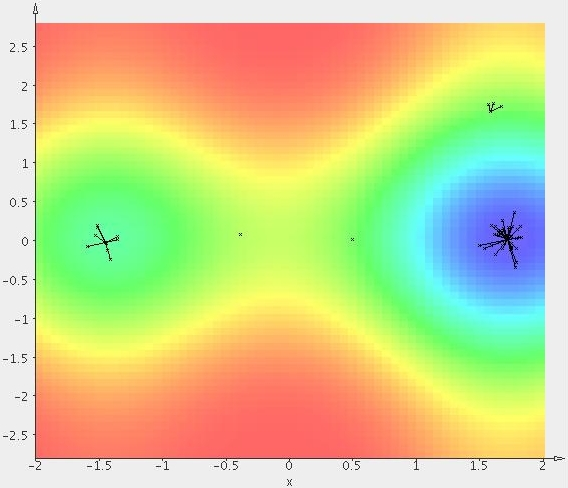
\includegraphics[width=0.49\columnwidth]{pics/fm0-cbn-500}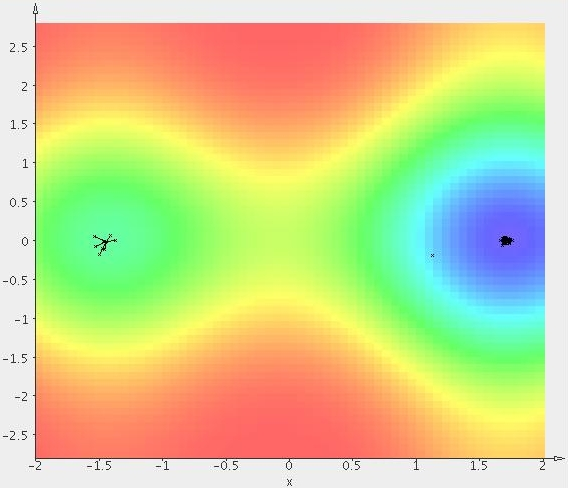
\includegraphics[width=0.49\columnwidth]{pics/fm0-cbn-1500}

\caption{Exemplary states of CBN on the simple bimodal FM0Problem.\label{fig:Exemplary-states-of-CBN}}
\end{figure}


The FM0Problem is of course very simple, 2-dimensional and having
only two optima in the defined range. For harder problems, a few thousand
evaluations will not suffice, and for highly multi-modal target functions,
e.g. if there are thousands or tens of thousands of local optima,
things get really tough. The current implementation of CBN is able
to find more optima than the population size defined, because it is
able to reinitialize a converged cluster during a run, saving a representative
to an archive. But for problems with a lot of deceptive optima, it
might also be a good strategy to concentrate on finding one global
optimum, and, as it won't be found in most of the runs, look at the
results of the single-run solution set.